\begin{frame}{Repère orthogonal 2D}
    \small
    Un repère orthogonal 2D est une croix orientée par un angle $\theta$.
    \newline
    \newline
    \begin{minipage}{0.46\textwidth}
        \centering
        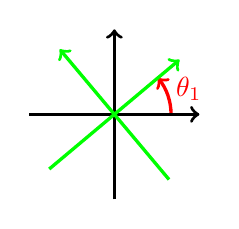
\begin{tikzpicture}[very thick, scale=.9]
            \draw[->, red] (.8, 0) arc (0:40:.8) node[right,pos=.66] {$\theta_1$};
            \draw[->] (180:1.2) -- (0:1.2);
            \draw[->] (-90:1.2) -- (90:1.2);
            \draw[->, green] (220:1.2) -- (40:1.2);
            \draw[->, green] (310:1.2) -- (130:1.2);
        \end{tikzpicture}
    \end{minipage}
    \hfill
    \begin{minipage}{0.46\textwidth}
        \centering
        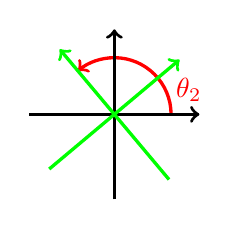
\begin{tikzpicture}[very thick, scale=.9]
            \draw[->, red] (.8, 0) arc (0:130:.8) node[right,pos=.2] {$\theta_2$};
            \draw[->] (180:1.2) -- (0:1.2);
            \draw[->] (-90:1.2) -- (90:1.2);
            \draw[->, green] (220:1.2) -- (40:1.2);
            \draw[->, green] (310:1.2) -- (130:1.2);
        \end{tikzpicture}
    \end{minipage}
    
    \vfill
    
    \small
    Une croix étant $\pi/2$-périodique, nous la représentons par $(X, Y) = (\cos4\theta, \sin4\theta)$ pour éviter les problèmes de périodicité.
    \newline
    \newline
    \begin{minipage}{0.4\textwidth}
        \centering
        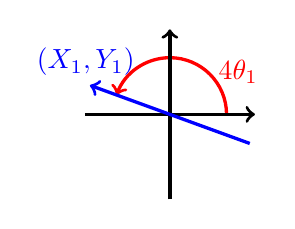
\begin{tikzpicture}[very thick, scale=.9]
            \draw[->, red] (.8, 0) arc (0:160:.8) node[right,pos=.3] {$4\theta_1$};
            \draw[->] (180:1.2) -- (0:1.2);
            \draw[->] (-90:1.2) -- (90:1.2);
            \draw[->, blue] (340:1.2) -- (160:1.2) node[right,pos=1.4] {$(X_1, Y_1)$};
        \end{tikzpicture}
    \end{minipage}
    \hfill
    \begin{minipage}{0.53\textwidth}
        \centering
        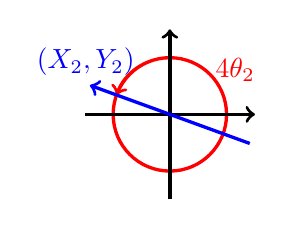
\begin{tikzpicture}[very thick, scale=.9]
            \draw[->, red] (.8, 0) arc (0:520:.8) node[right,pos=.1] {$4\theta_2$};
            \draw[->] (180:1.2) -- (0:1.2);
            \draw[->] (-90:1.2) -- (90:1.2);
            \draw[->, blue] (340:1.2) -- (160:1.2) node[right,pos=1.4] {$(X_2, Y_2)$};
        \end{tikzpicture}
    \end{minipage}
\end{frame}
\begin{frame}{Champ de repère 2D plat}
    \centering
    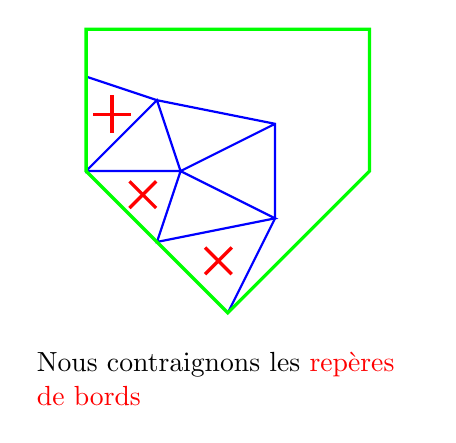
\begin{tikzpicture}[very thick, scale=.6]
    \node[text width=.4\linewidth] at (3, -1.4) {Nous contraignons les \color{red} repères de bords};
    \draw[blue, thick] (3, 0) -- (4, 2) -- (4, 4) -- (1.5, 4.5) -- (0, 5) -- (0, 3) -- (1.5, 4.5) -- (2, 3) -- (4, 4);
    \draw[blue, thick] (0, 3) -- (2, 3) -- (1.5, 1.5) -- (4, 2) -- (2, 3);
    \draw[green] (0, 3) -- (3, 0) -- (6, 3) -- (6, 6) -- (0, 6) -- cycle;
    \draw[red] (.55, 4.2) {}++ (0:.4) --+ (180:.8);
    \draw[red] (.55, 4.2) {}++ (90:.4) --+ (270:.8);
    \draw[red] (1.2, 2.5) {}++ (45:.4) --+ (225:.8);
    \draw[red] (1.2, 2.5) {}++ (135:.4) --+ (315:.8);
    \draw[red] (2.8, 1.1) {}++ (45:.4) --+ (225:.8);
    \draw[red] (2.8, 1.1) {}++ (135:.4) --+ (315:.8);
    \end{tikzpicture} \pause \qquad
    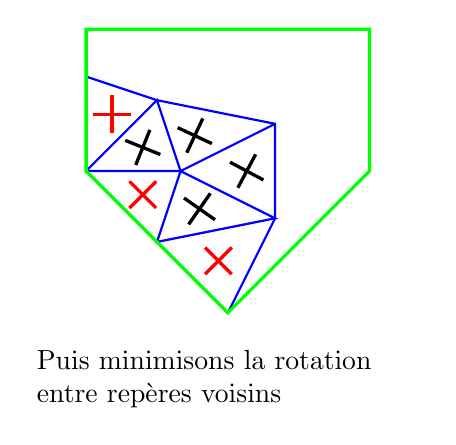
\begin{tikzpicture}[very thick, scale=.6]
    \node[text width=.4\linewidth] at (3, -1.4) {Puis minimisons la rotation entre repères voisins};
    \draw[blue, thick] (3, 0) -- (4, 2) -- (4, 4) -- (1.5, 4.5) -- (0, 5) -- (0, 3) -- (1.5, 4.5) -- (2, 3) -- (4, 4);
    \draw[blue, thick] (0, 3) -- (2, 3) -- (1.5, 1.5) -- (4, 2) -- (2, 3);
    \draw[green] (0, 3) -- (3, 0) -- (6, 3) -- (6, 6) -- (0, 6) -- cycle;
    \draw[red] (.55, 4.2) {}++ (0:.4) --+ (180:.8);
    \draw[red] (.55, 4.2) {}++ (90:.4) --+ (270:.8);
    \draw[red] (1.2, 2.5) {}++ (45:.4) --+ (225:.8);
    \draw[red] (1.2, 2.5) {}++ (135:.4) --+ (315:.8);
    \draw[red] (2.8, 1.1) {}++ (45:.4) --+ (225:.8);
    \draw[red] (2.8, 1.1) {}++ (135:.4) --+ (315:.8);
    \draw[] (2.4, 2.2) {}++ (55:.4) --+ (235:.8);
    \draw[] (2.4, 2.2) {}++ (145:.4) --+ (325:.8);
    \draw[] (3.4, 3.) {}++ (62:.4) --+ (242:.8);
    \draw[] (3.4, 3.) {}++ (152:.4) --+ (332:.8);
    \draw[] (1.2, 3.5) {}++ (68:.4) --+ (248:.8);
    \draw[] (1.2, 3.5) {}++ (158:.4) --+ (338:.8);
    \draw[] (2.3, 3.75) {}++ (65:.4) --+ (245:.8);
    \draw[] (2.3, 3.75) {}++ (155:.4) --+ (335:.8);
    \end{tikzpicture}
\end{frame}
\begin{frame}{Champ de repère 2D plat}
    \small
    Pour optimiser un champ de repère 2D plat sans problème de périodicité, nous optimisons 
    les vecteurs de représentations $(X, Y)$:
    \small{
    \begin{equation*}
    \begin{array}{ll}
    \underset{X, Y}{\argmin} & \underset{t \in T}{\displaystyle\sum} \underset{t' \in \mathcal{N}(t)}{\displaystyle\sum} \left|\left|\ \begin{pmatrix} X_{t'}\\ Y_{t'}\end{pmatrix} - \begin{pmatrix} X_{t}\\ Y_{t}\end{pmatrix} \right|\right|^2, \\
    \text{sous contrainte: } & \forall t \in T_b, \begin{pmatrix} X_{t}\\ Y_{t}\end{pmatrix} = \begin{pmatrix} \cos4\eta_t\\ \sin4\eta_t\end{pmatrix}.
    \end{array}
    \end{equation*}
    }
    Puis nous retrouvons les angles $\theta$ du champ de repère:
    $$ \forall t \in T,\ \  \theta_t = \frac{1}{4}\tan^{-1}\frac{Y_t}{X_t}$$

\end{frame}

\begin{frame}{Comparaison de repères dans deux plans différents}
    \begin{center}
    \begin{tikzpicture}[scale=2, transform shape]
    \coordinate (A) at (0,0);
    \coordinate (B) at (2,0);
    \coordinate (C) at (1,1.7);
    \coordinate (D) at (3,0.85);
    
    % Calculate the center of each triangle
    \coordinate (Center1) at ($ 0.333*(A) + 0.333*(B) + 0.333*(C) $);
    \coordinate (Center2) at ($ 0.333*(C) + 0.333*(B) + 0.333*(D) $);
    \coordinate (Ref1) at ($(Center1) + 0.5*(C) - 0.5*(B)$);
    \coordinate (Ref2) at ($(Center2) + 0.5*(C) - 0.5*(B)$);
    \coordinate (Ref3) at ($(Center1) - 0.5*(C) + 0.5*(B)$);
    \coordinate (Ref4) at ($(Center2) - 0.5*(C) + 0.5*(B)$);
    \coordinate (Ref5) at ($(Center1) + 0.5*(A) - 0.5*(B)$);
    \coordinate (Ref6) at ($(Center1) - 0.5*(A) + 0.5*(B)$);
    
    % Draw the shadows first
    \draw[drop shadow={shadow xshift=1.ex,shadow yshift=-1.ex}] (A) -- (B) -- (C) -- cycle;
    \draw[drop shadow={shadow xshift=1.ex,shadow yshift=-1.ex}] (B) -- (D) -- (C) -- cycle;
    
    % Then draw the triangles
    \fill[blue, opacity=0.3, shading=ball, ball color=blue] (A) -- (B) -- (C) -- cycle;
    \fill[red, opacity=0.3, shading=ball, ball color=red] (B) -- (D) -- (C) -- cycle;
    
    % Draw the green crosses
    \begin{scope}[overlay]
        \node at (Center1) [rotate=30, green, scale=2] {$\times$};
        \node at (Center2) [rotate=10, green, scale=2] {$\times$};
    \end{scope}

    % Highlight the common edge
    \draw[ultra thick] (B) -- (C);
    

    % Calculate the start of the arcs (cross arm ends)
    \coordinate (StartArc1) at ($(Center1) + (30+45:0.25)$);
    \coordinate (StartArc2) at ($(Center2) + (10+45:0.25)$);
    \coordinate (Arriv1) at ($(Center1) + 0.125*(C) - 0.125*(B)$);
    \coordinate (Arriv2) at ($(Center2) + 0.125*(C) - 0.125*(B)$);

    % Add the angles
    \only<2-2>{
        \draw[->] (StartArc1) to[bend right=30] (Arriv1);    
        \node[scale=0.8] at ($(Center1)!0.5!(StartArc1) + (0.,0.35)$) {$\theta_1$};
    }
    \only<2-3>{
        % Add the dotted lines
        \draw[dotted] (Ref3) -- (Ref1);
        \draw[dotted] (Ref4) -- (Ref2);

        \draw[->] (StartArc2) to[bend right=30] (Arriv2);
        \node[scale=0.8] at ($(Center2)!0.5!(StartArc2) + (0.,0.35)$) {$\theta_2$};
    }
    
    \coordinate (StartArc3) at ($(Center1) + (30+45:0.25)$);
    \coordinate (Arriv3) at ($(Center1) - 0.14*(A) + 0.14*(B)$);
    \only<3-3>{
        % Add the dotted lines
        \draw[dotted] (Ref5) -- (Ref6);
        
        % Calculate the start of the arcs (cross arm ends)
        
        % Add the angles
        \draw[->] (StartArc3) to[bend left=30] (Arriv3);
        \node[scale=0.8] at ($(Center1)!0.5!(StartArc3) + (0.25,0.2)$) {$\theta_1$};

        % Add alpha angle
        \coordinate (alphaStart) at ($(Center1) + 0.3*(C) - 0.3*(B)$);
        \coordinate (alphaEnd) at ($(Center1) - 0.3*(A) + 0.3*(B)$);
        \draw[->,red] (alphaStart) to[bend left=40] (alphaEnd);
        \node[red,scale=0.8] at ($(Center1)!0.5!(StartArc3) + (0.,0.5)$) {$\alpha_1$};
    }

    \only<4-4>{
        \draw[dotted] (Ref4) -- (Ref2);
        \draw[dotted] (Ref5) -- (Ref6);
        \draw[->] (StartArc3) to[bend left=30] (Arriv3);
        \node[scale=0.8] at ($(Center1)!0.5!(StartArc3) + (0.25,0.2)$) {$\theta_{t}$};
        \draw[->] (StartArc2) to[bend right=30] (Arriv2);
        \node[scale=0.8] at ($(Center2)!0.5!(StartArc2) + (0.,0.35)$) {$\theta_{t'}$};
         % Add omega
        \node[blue, scale=0.8] at ($(B)!0.3!(C)$) {$\omega_{tt'}$};
    }
    
    \end{tikzpicture}
    \newline
    \only<1-1>{
        \newline
        Nous utilisons l'arête commune pour comparer les angles des repères par rapport à une même référence.
        %Problème: comment comparer des repères se situant dans deux plans différents ?\\ 
        %Nous allons utiliser l'arête partagée par les deux triangles comme référence d'angle.
    }
    \only<2-2>{
        Rotation entre les deux repères: $\theta_2 - \theta_1 \pmod{\pi/2}$
    }
    \only<3-3>{
        Rotation entre les deux repères: $\theta_2 - \theta_1 + \alpha_1 \pmod{\pi/2}$\\
        Ou plus généralement: $\theta_2 - \theta_1 - \alpha_2 + \alpha_1 \pmod{\pi/2}$
    }
    \only<4-4>{
        \newline
        Pour chaque paire de triangles adjacents $t, t'$, on définit:
        $$\omega_{tt'} = - \omega_{t't} = \alpha_{t'} - \alpha_{t}$$
        La rotation entre les repères de $t$ et $t'$ devient: 
        $$
            \theta_{t'} - \theta_{t} - \omega_{tt'} \pmod{\pi/2}
        $$
    }
    \end{center}


\end{frame}

\iffalse
\begin{frame}{Champ de repère 2D surfacique}
    \small
    Dans le cas surfacique, nous voulons minimiser les rotations:
    $$
        \theta_{t'} - \theta_{t} - \omega_{tt'} \pmod{\pi/2}
    $$

    Le problème d'optimisation devient alors :
    \small{
    \begin{equation*}
    \begin{array}{ll}
    \underset{X, Y}{\argmin} & \underset{t \in T}{\displaystyle\sum} \underset{t' \in \mathcal{N}(t)}{\displaystyle\sum} \left|\left|\ \begin{pmatrix} X_{t'}\\ Y_{t'}\end{pmatrix} - \begin{pmatrix}\cos4\omega_{tt'} & -\sin4\omega_{tt'} \\ \sin4\omega_{tt'} & \cos4\omega_{tt'} \end{pmatrix} \begin{pmatrix} X_{t}\\ Y_{t}\end{pmatrix} \right|\right|^2, \\
    \text{sous contrainte: } & \forall t \in T_b, \begin{pmatrix} X_{t}\\ Y_{t}\end{pmatrix} = \begin{pmatrix} \cos4\eta_t\\ \sin4\eta_t\end{pmatrix}.
    \end{array}
    \end{equation*}
    }
\end{frame}

\begin{frame}
    \frametitle{Maillages quadrilatères surfaciques}
    \begin{figure}
    \centering
    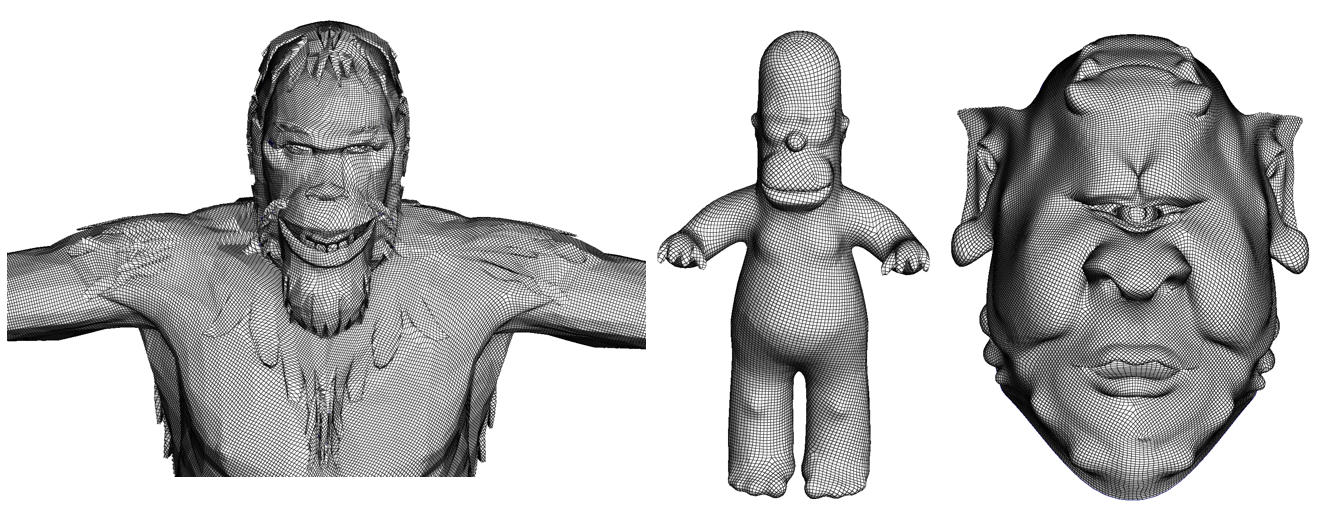
\includegraphics[width=\textwidth]{img/new_images/CG_models.PNG}
    \caption{Exemple de maillages quadrilatères surfaciques}
    \end{figure}
\end{frame}
\fi

\begin{frame}{Problèmes des bords à petits angles}

    \begin{center}
    \begin{tabular}{c|c|c|c|c}
    % First row: angle text
    $\alpha_v=10^{\circ}$ & $\alpha_v=90^{\circ}$ & $\alpha_v=180^{\circ}$ & $\alpha_v=270^{\circ}$ & $\alpha_v=350^{\circ}$ \\
    \hline
    % Second row: TikZ diagrams
    \begin{minipage}{0.14\textwidth}
    \centering
    \begin{tikzpicture}[scale=0.2]
    % Lines forming a 10° angle
    \draw (0,0) -- (0,3);
    \draw (0,0) -- ({3*sin(10)},{3*cos(10)});
    \node[rotate=40, green, scale=2] at (0.2,2) {$\times$}; % Added cross
    \end{tikzpicture}
    \end{minipage}
    &
    \begin{minipage}{0.14\textwidth}
    \centering
    \begin{tikzpicture}[scale=0.2]
    \only<2-4> {
    \draw[red] (0.0,0.0) rectangle (3.0,3.0); % Added quadrilateral
    }
    % Lines forming a 90° angle
    \draw (0,0) -- (0,3);
    \draw (0,0) -- (3,0);
    \node[rotate=45, green, scale=2] at (1.5,1.5) {$\times$}; % Added cross
    \end{tikzpicture}
    \end{minipage}
    &
    \begin{minipage}{0.17\textwidth}
    \centering
    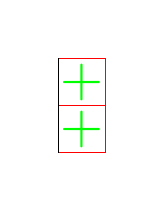
\begin{tikzpicture}[scale=0.2]
    \only<2-4> {
    \draw[red] (0.0,0.0) rectangle (3.0,3.0); % Added quadrilateral
     \draw[red] (0.0,-3.0) rectangle (3.0,0.0); % Added quadrilateral
    }
    % Lines forming a 180° angle
    \draw (0,0) -- (0,3);
    \draw (0,0) -- (0,-3);
    \node[rotate=45, green, scale=2] at (1.5,1.5) {$\times$}; % Added cross
    \node[rotate=45, green, scale=2] at (1.5,-1.5) {$\times$}; % Added cross
    \end{tikzpicture}
    \end{minipage}
    &
    \begin{minipage}{0.17\textwidth}
    \centering
    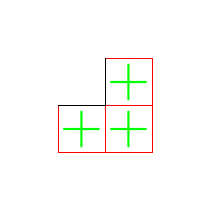
\begin{tikzpicture}[scale=0.2]
    % Lines forming a 270° angle
    \only<2-4> {
     \draw[red] (0.0,0.0) rectangle (3.0,3.0); % Added quadrilateral
     \draw[red] (0.0,-3.0) rectangle (3.0,0.0); % Added quadrilateral
     \draw[red] (-3.0,-3.0) rectangle (0.0,0.0); % Added quadrilateral
    }
    \draw (0,0) -- (0,3);
    \draw (0,0) -- (-3,0);
    \node[rotate=45, green, scale=2] at (1.5,1.5) {$\times$}; % Added cross
    \node[rotate=45, green, scale=2] at (1.5,-1.5) {$\times$}; % Added cross
    \node[rotate=45, green, scale=2] at (-1.5,-1.5) {$\times$}; % Added cross
    \end{tikzpicture}
    \end{minipage}
    &
    \begin{minipage}{0.17\textwidth}
    \centering
    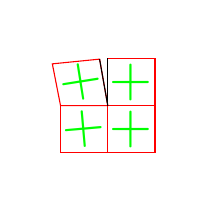
\begin{tikzpicture}[scale=0.2]
    % Lines forming a 350° angle
    \only<2-4> {
     \draw[red] (0.0,0.0) rectangle (3.0,3.0); % Added quadrilateral
     \draw[red] (0.0,-3.0) rectangle (3.0,0.0); % Added quadrilateral
     \draw[red] (-3.0,-3.0) rectangle (0.0,0.0); % Added quadrilateral
     \draw[red] (-3.0,0.0) -- (0.0,0.0) -- ({3*sin(350)},{3*cos(350)}) -- ({3*sin(350)-3},{3*cos(350) - 0.3}) -- cycle; % Added parallelogram
    }
    \draw (0,0) -- (0,3);
    \draw (0,0) -- ({3*sin(350)},{3*cos(350)});
    \node[rotate=45, green, scale=2] at (1.5,1.5) {$\times$}; % Added cross
    \node[rotate=45, green, scale=2] at (1.5,-1.5) {$\times$}; % Added cross
    \node[rotate=50, green, scale=2] at (-1.5,-1.5) {$\times$}; % Added cross
    \node[rotate=54, green, scale=2] at (-1.7,1.5) {$\times$}; % Added cross
    \end{tikzpicture}
    \end{minipage}
    \end{tabular}
    
    \only<3-4>{
        \vspace{0.3cm}
        Un champ de repère orthogonal produit un maillage quadrilatère de valence de bord: $$k_v = \text{arrondi} \left( \frac{\alpha_v}{90} \right)$$
    }
    \only<4-4>{
        Problème: pour $\alpha_v < 45^\circ$, on obtient une valence $k_v = 0$ qui fait échouer la méthode. %le sommet de bord est donné de valence 0, ce qui fait échouer la méthode.
    }
    \end{center}
    
\end{frame}

\begin{frame}{Problèmes avec les modèles CAO}
    \begin{center}
        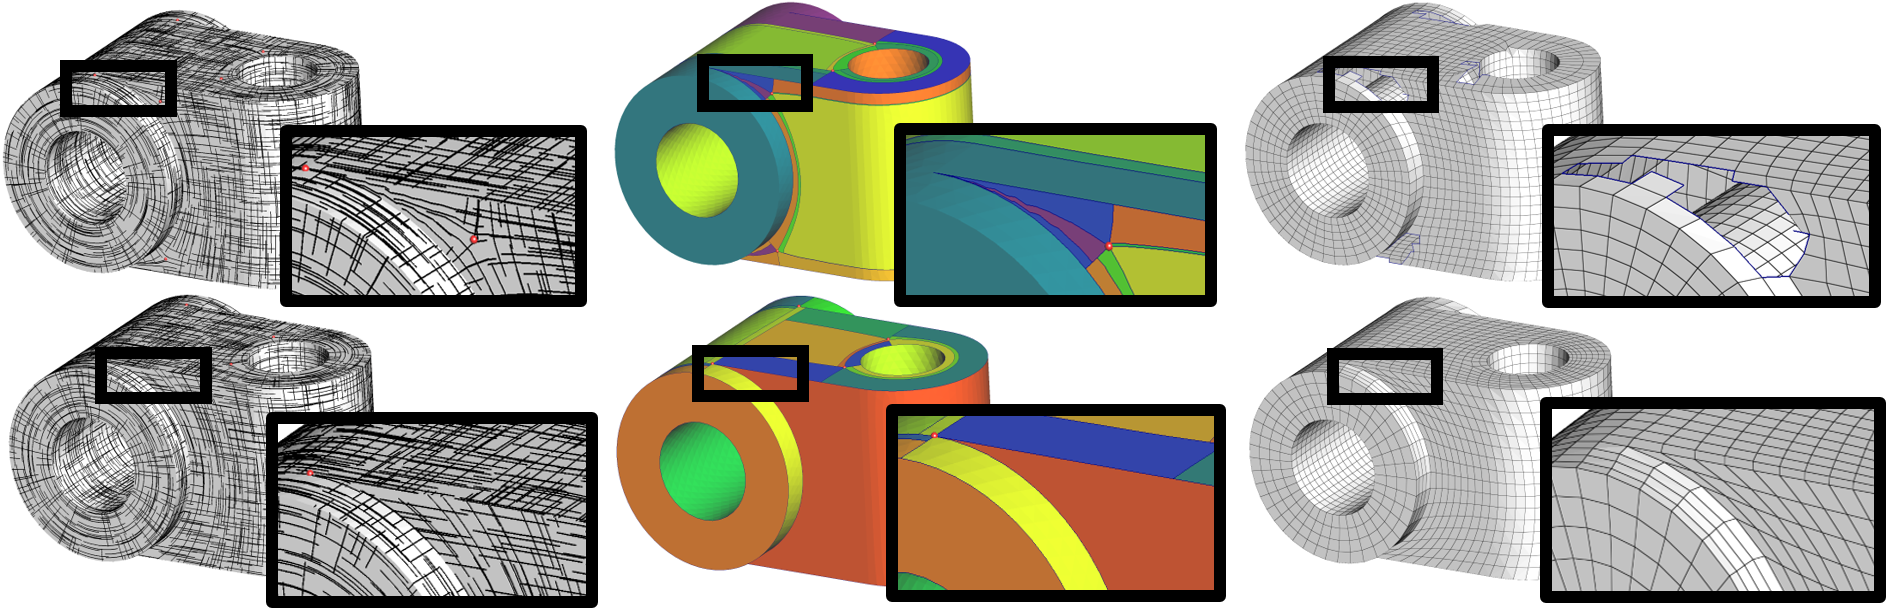
\includegraphics[width=0.9\linewidth]{img/cadff/teaser2}
        \small{
            \textit{Produire un champ de repère qui a une rotation minimale sur un modèle CAO ne suffit pas toujours pour obtenir un maillage quad de qualité (haut). 
            Notre algorithme permet de gérer les cas où il y a des configurations d'arêtes caractéristiques formant des petits angles (bas).}
        }
    \end{center}
\end{frame}
    
\begin{frame}{Intuition de la contribution}
    \begin{center}
        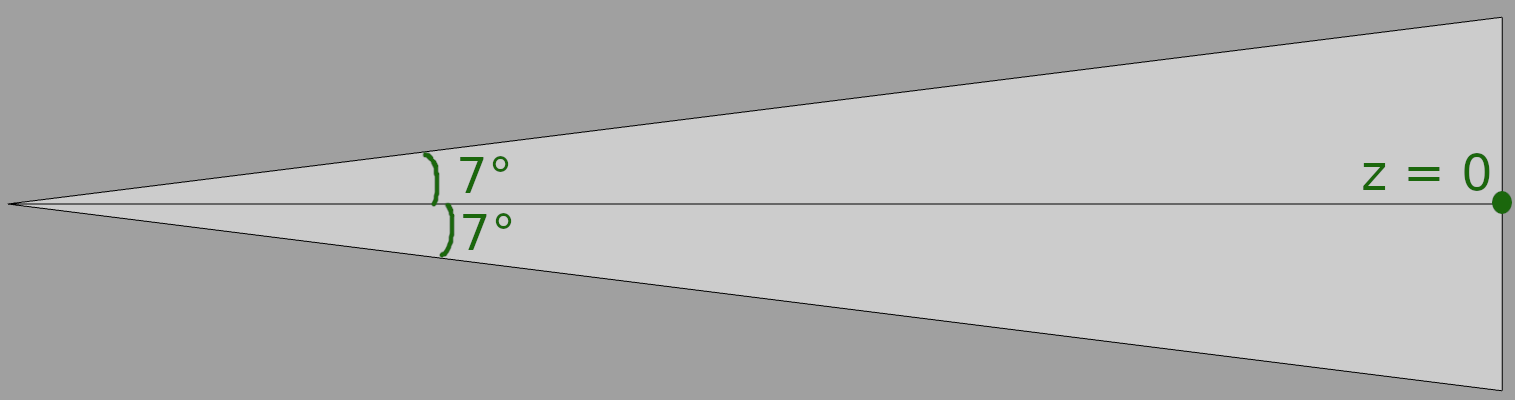
\includegraphics[width=0.9\linewidth]{img/new_images/flat_tri_annot.png}
        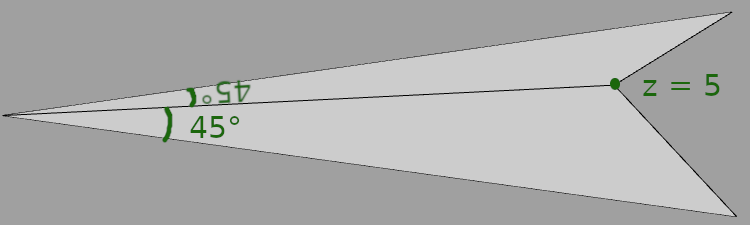
\includegraphics[width=0.9\linewidth]{img/new_images/surface_tri_annot.png}
        \small{
            \textit{Modifier la définition du transport parallèle permet de transformer les petits angles en angles de 90°.}
        }
    \end{center}
\end{frame}

\begin{frame}{Modification de la définition du transport parallèle pour empêcher les petits angles}

    \begin{center}
    \begin{tikzpicture}[scale=1]
    % Triangle 1
    \draw[fill=blue!20] (0,0) -- (8,0) -- (8,1) -- cycle;
    
    % Triangle 2
    \draw[fill=red!20] (0,0) -- (8,0) -- (8,-1) -- cycle;
    
    % Angle arc for α_v
    %\draw[->] (1,-0.15) arc (0:15:1);  % Arc now goes in counterclockwise direction
    
    \only<1>{
        \node at ($ (2,0) $) {$\alpha_v = 15^{\circ}$}; % Shifted to the right
        \draw[->, blue] ($ (8,0) + (0,-0.5) $) to [bend left=45] ($ (8,0) + (0,0.5) $); % Flèche going from bottom to top
        \node[blue] at ($ (8,0) + (1,0) $) {$\omega = 0^{\circ}$};
    }
    \only<2>{
        \node at ($ (2,0) $) {$\alpha_v = 90^{\circ}$}; % Shifted to the right
        \draw[->, blue] ($ (8,0) + (0,-0.5) $) to [bend left=45] ($ (8,0) + (0,0.5) $); % Flèche going from bottom to top
        \node[blue] at ($ (8,0) + (1,0) $) {$\ \ \omega + \gamma = 75^{\circ}$};
    }
    
    \end{tikzpicture}
    \end{center}
    
\end{frame}
    
    
\begin{frame}{Diffusion of $\gamma$}
    
    \begin{figure}
    \centering
    \begin{subfigure}{.3\textwidth}
      \centering
      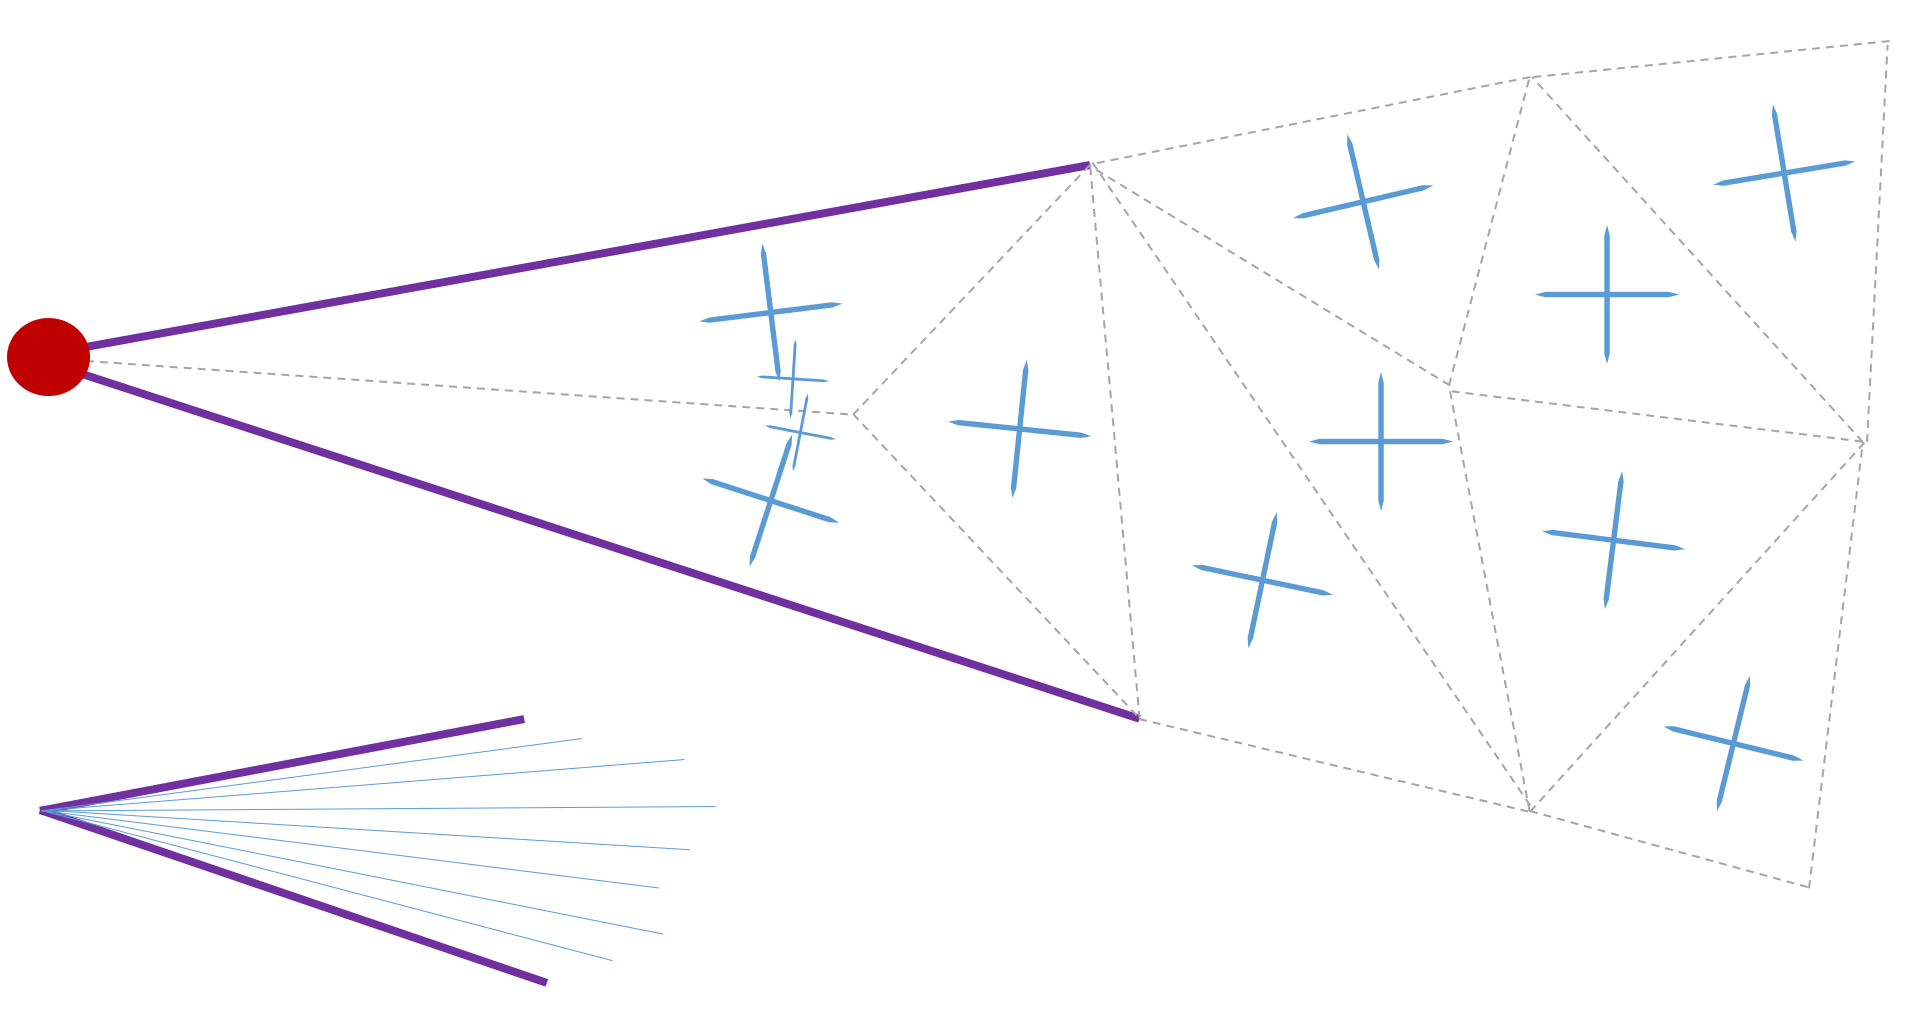
\includegraphics[width=0.9\linewidth]{img/cadff/sharp0}
      \caption{Champ le plus lisse}
    \end{subfigure}%
    \hspace{0.03\textwidth}
    \begin{subfigure}{.3\textwidth}
      \centering
      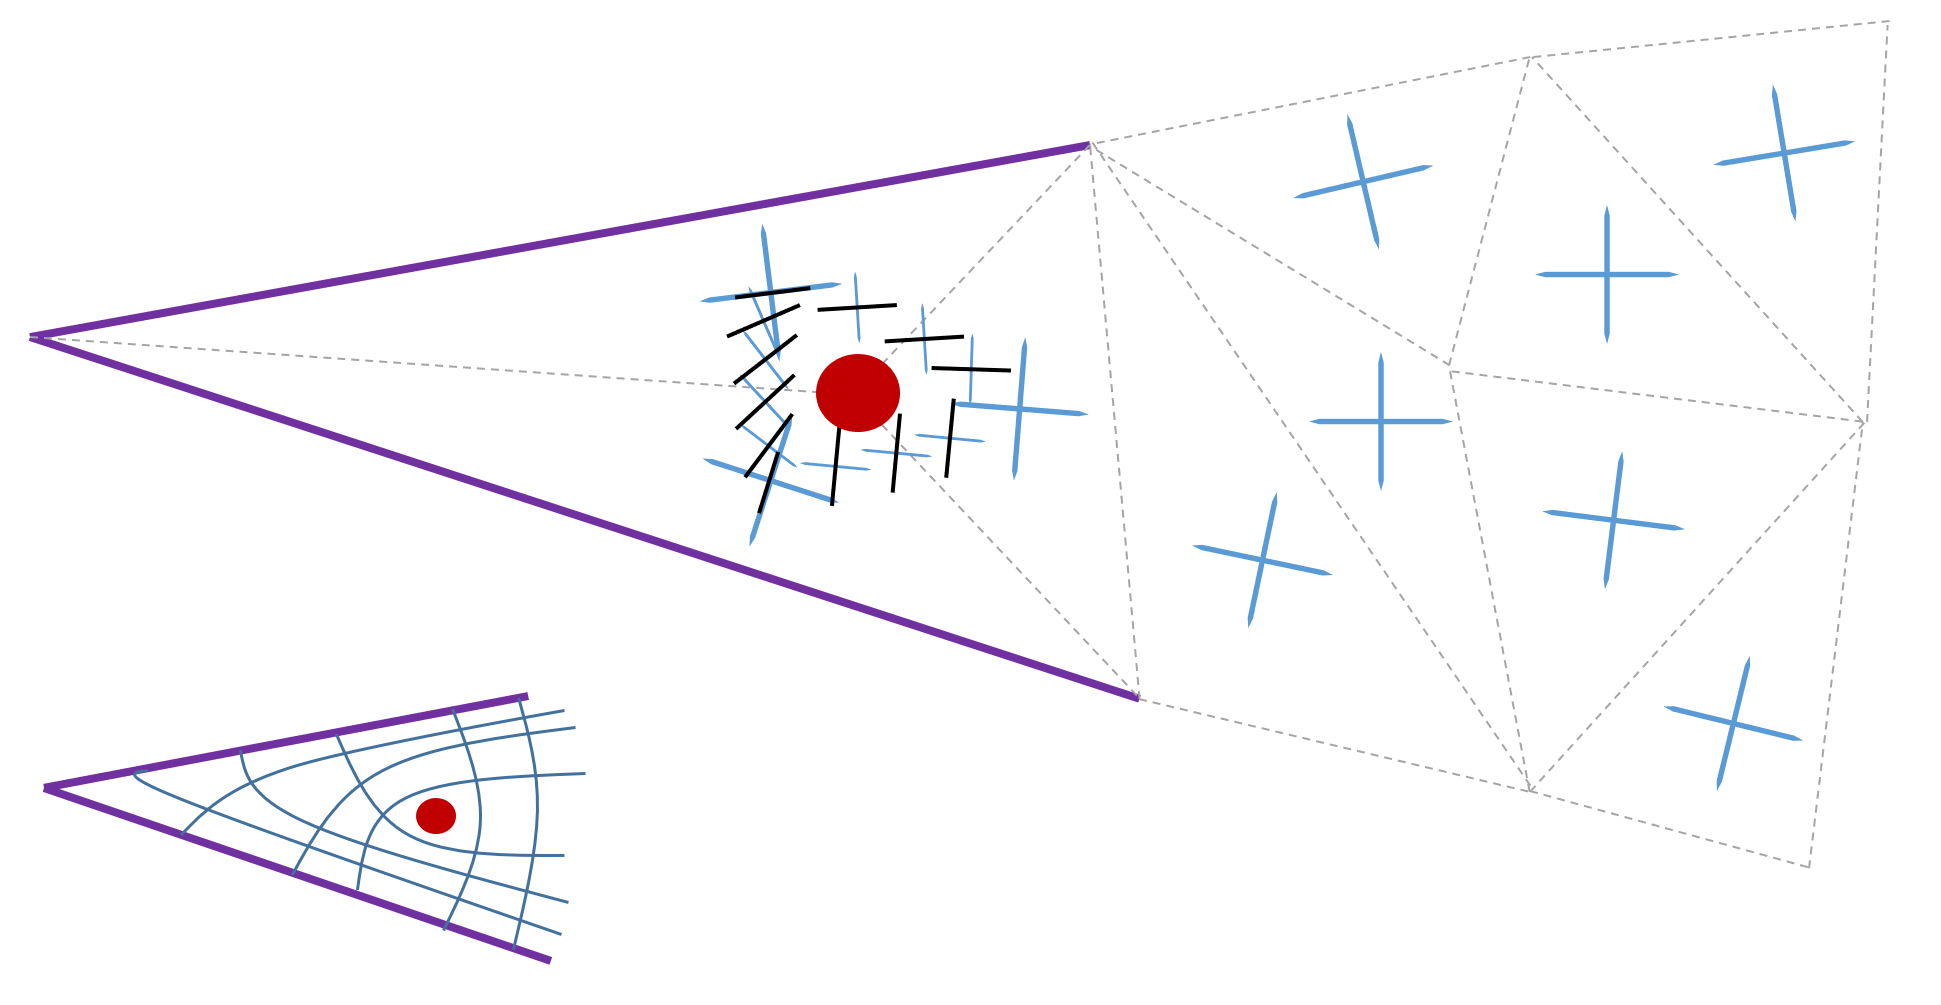
\includegraphics[width=0.9\linewidth]{img/cadff/sharp1}
      \caption{Singularité sur le 1-voisinage}
    \end{subfigure}
    \hspace{0.03\textwidth}
    \begin{subfigure}{.3\textwidth}
      \centering
      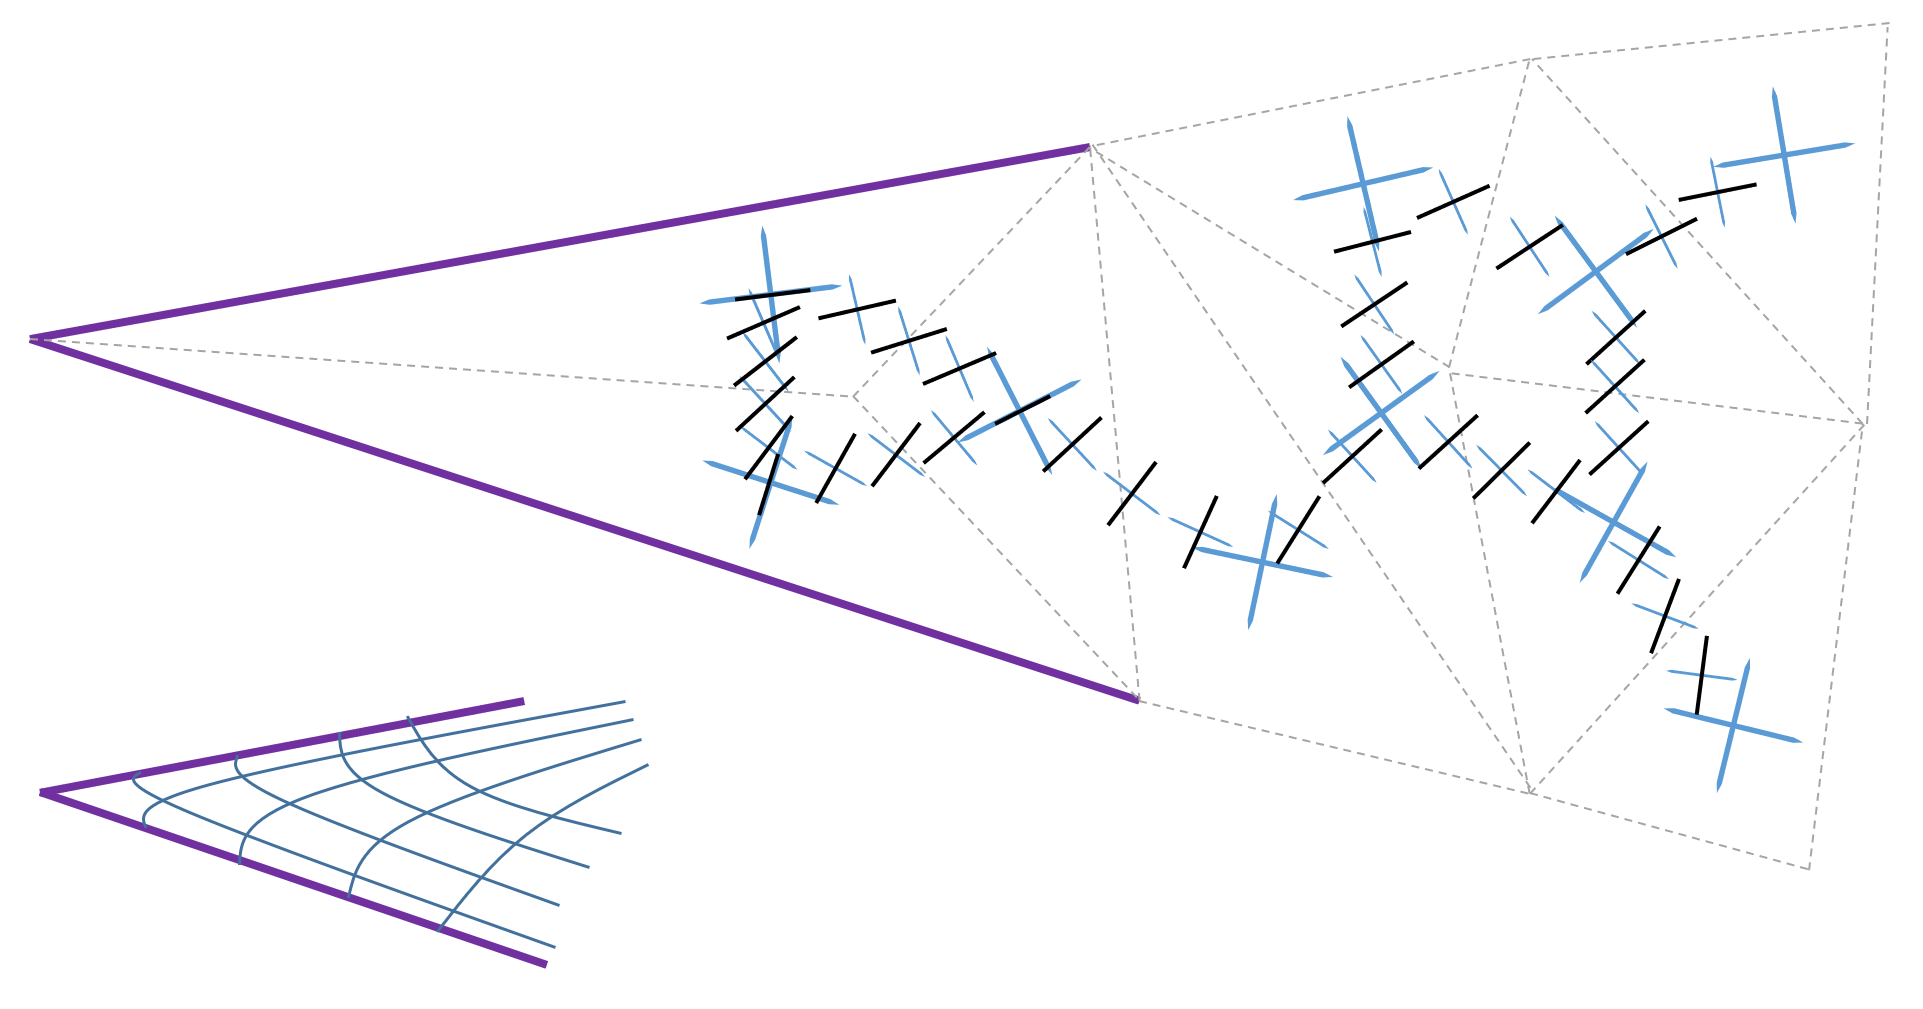
\includegraphics[width=0.9\linewidth]{img/cadff/sharp2}
      \caption{Propagation globale de la courbure}
    \end{subfigure}%
    \caption{Sur un sommet de coin pointu, le champ le plus lisse produit des lignes de quads qui se concentrent au niveau du sommet (a). Une correction locale peut 
    résoudre ce problème (b), mais la propagation de la courbure du champ est ce qui permet d'obtenir les lignes de quads les plus utilisables (c).}
    \label{fig:cadff:sharp2}
    \end{figure}
    
\end{frame}
    
\begin{frame}{Comment calculer $\gamma$}

    Au lieu de rendre singulier le sommet le plus proche, il peut être préférable de déplacer le sommet singulier plus loin.
    
    Pour y parvenir, nous proposons une méthode d'optimisation en deux étapes pour déterminer $\gamma$ :
    \begin{itemize}
        \item Calcul de $K(v)$ pour chaque sommet $v$, avec l'objectif de minimiser $\sum_v K(v)^2$ tout en s'assurant que $\sum_v K(v)=0$. Pour les sommets de coin pointus $v$, $K(v) = \pi/2 - \theta_v$.
        \item Minimisation de $\argmin \sum_{tt'}|\gamma_{tt'}|^2$ sous la contrainte $\mathrm{d}\gamma(v) = K(v)$. L'existence d'une solution est garantie par la contrainte $\sum_v K(v)=0$.
    \end{itemize}
    
    Cela permet de propager la modification du transport parallèle plus loin que seulement sur les arêtes adjacentes au sommet problématique $v$.
    
\end{frame}

\begin{frame}{Optimisation et calcul des correspondances}

    \scriptsize
    \begin{equation}
        \begin{array}{ll}
        \underset{X, Y}{\argmin} & \underset{t \in T}{\displaystyle\sum} \underset{t' \in \mathcal{N}(t)}{\displaystyle\sum} \left|\left|\ \begin{pmatrix} X_{t'}\\ Y_{t'}\end{pmatrix} - \begin{pmatrix}\cos4(\omega_{tt'} + \gamma_{tt'}) & -\sin4(\omega_{tt'} + \gamma_{tt'}) \\ \sin4(\omega_{tt'} + \gamma_{tt'}) & \cos4(\omega_{tt'} + \gamma_{tt'}) \end{pmatrix} \begin{pmatrix} X_{t}\\ Y_{t}\end{pmatrix} \right|\right|^2, \\
        \text{sous : } & \forall t \in T_b, \begin{pmatrix} X_{t}\\ Y_{t}\end{pmatrix} = \begin{pmatrix} \cos4\eta_t\\ \sin4\eta_t\end{pmatrix}.
        \end{array}
        \label{eq:cadff_ff_2D_surface_optim}
    \end{equation}
    
    \[\small
    \text{Correspondance: } p_{tt'} = round\left(\frac{\theta_{t'} - \theta_t - \omega_{tt'} - \gamma_{tt'}}{\pi/2}\right)
    \]
    
    
\end{frame}